\chapter{Solving RL Problems using DP \cite{baeldung/cs/ml-value-iteration-vs-policy-iteration}}

\section{Value Iteration \cite{baeldung/cs/ml-value-iteration-vs-policy-iteration}}

First, we start with a random value function $V(s)$. At each step, we update it:

\[
    V(s) = \max_{a} \sum_{s',r'}p(s', r|s,a)[r+\gamma V(s')]
\]

\begin{algorithm}[H]
    \caption{Reinforcement Learning - DP: Value Iteration Algorithm}
    
    \textbf{Data}: $\theta$: a small number\\
    \textbf{Result}: $\pi$: a deterministic policy s.t. $\pi \approx \pi_*$\\

    \SetKwFunction{FValueIteration}{ValueIteration}
    \SetKwProg{Fn}{Function}{:}{}
    \Fn{\FValueIteration{}}{
        \Comment{Initialization}
        Initialize $V(s)$ arbitrarily, except $V(terminal)$\;
        $V(terminal) \leftarrow 0$\;
        \Comment{Loop until convergence}
        $\Delta \leftarrow 0$\;
        \While{$\Delta < \theta$}{
            \ForEach{ $s \in S$}{
                $v \leftarrow V(s)$\;
                $V(s) \leftarrow \displaystyle\max_a \displaystyle\sum_{s',r'} p(s',r|s,a)[r+\gamma V(s')]$\;
            }
        }
        \Comment{Return optimal policy}
        return $\pi$ s.t. $\pi(s) = \displaystyle\arg\max_a \displaystyle\sum_{s',r'} p(s',r|s,a)[r+\gamma V(s')]$\;
    }
\end{algorithm}

The update step is very similar to the update step in the policy iteration algorithm. Moreover, the only difference is that in the value iteration algorithm, we take the maximum number of possible actions.

Instead of evaluating and then improving, the value iteration algorithm updates the state value function in a single step. In particular, this is possible by calculating all possible rewards by looking ahead.

Finally, the value iteration algorithm is guaranteed to converge to the optimal values.




\section{Policy Iteration \cite{baeldung/cs/ml-value-iteration-vs-policy-iteration}}

In policy iteration, we start by choosing an arbitrary policy $\pi$. Then, we iteratively evaluate and improve the policy until convergence.

\begin{enumerate}
    \item evaluate a policy $\pi(s)$ by calculating the state value function $V(s)$:
    \[
        V(s) = \sum_{s',r'}p(s', r|s,\pi(s))[r+\gamma V(s')]
    \]
    \item calculate the improved policy by using a one-step look-ahead to replace the initial policy $\pi(s)$:
    \[
        \pi(s) = \arg\max_{a} \sum_{s',r'} p(s', r|s,a)[r+\gamma V(s')]
    \]
    $r$ is the reward generated by taking action $a$, $\gamma$ is a \textbf{discount factor} for future rewards, and $p$ is the transition probability.
    \item we don’t care about the initial policy $\pi_0$ being optimal or not. Additionally, during the execution, we concentrate on improving it on every iteration by repeating policy evaluation and policy improvement steps. Furthermore, using this algorithm, we produce a chain of policies, where each policy is an improvement over the previous one:
    \[
        \pi_0 \xrightarrow[]{\text{E}} v_{\pi_0} \xrightarrow[]{\text{I}} \pi_1 \xrightarrow[]{\text{E}} v_{\pi_1} \xrightarrow[]{\text{I}} \pi_2 \xrightarrow[]{\text{E}} \dotsi \xrightarrow[]{\text{I}} \pi_* \xrightarrow[]{\text{E}} v_{*}
    \]
\end{enumerate}

At the start of the policy iteration algorithm, we randomly set a policy and initialize its state value. Furthermore, the next step is to evaluate the initial policy by calculating the state value function. Moreover, the policy evaluation is an iterative process that involves continuously updating the policy’s state value until it converges.

After we complete the policy evaluation process, we move to the policy improvement phase. The main aim of this phase is to generate a new policy that is better than the current policy.

Finally, we check convergence criteria to determine if the policy has converged. To check the algorithm’s convergence, we inspect the old and newly generated policies. In case of convergence, both policies have to be the same. On the other hand, if convergence hasn’t been achieved, we go back to the policy evaluation phase and update the policy’s state value continuously until it converges.

Since a finite MDP has a finite number of policies, the defined process is finite. In the end, converging an optimal policy $\pi_*$ and an optimal value function $v_*$ is guaranteed.

\begin{algorithm}[h!]
    \caption{Reinforcement Learning - DP: Policy Iteration Algorithm}

    \textbf{Data}: $\theta$: a small number, $\eta$: another small number and $\eta > 0$\\
    \textbf{Result}: $V$: a value function s.t. $V_t(s) \approx v_*$, $\pi$: a deterministic policy s.t. $\pi \approx \pi_*$\\

    \SetKwFunction{FPolicyIteration}{PolicyIteration}
    \SetKwProg{Fn}{Function}{:}{}
    \Fn{\FPolicyIteration{}}{
        \Comment{Initialization}
        Initialize $V(s)$ arbitrarily\;
        Randomly initialize policy $\pi(s)$\;
        
        \Comment{Policy Evaluation}
        $\Delta \gets \eta$\;
        \While{$\Delta > \theta$}{
            \ForEach{$s \in S$}{
                $v \leftarrow V(s)$\;
                $V(s) \leftarrow \sum_{s',r'} p(s',r \mid s,\pi(s))[r+\gamma V(s')]$\;
                $\Delta \leftarrow \max(\Delta,|v-V(s)|)$\;
            }
        }
    
        
        \Comment{Policy Improvement}
        policy-stable $\leftarrow true$\;
        \ForEach{$s \in S$}{
            old-action $\leftarrow \pi(s)$\;
            $\pi(s) \leftarrow \arg\max_a \sum_{s',r'} p(s',r|s,a)[r+\gamma V(s')]$\;
            \If{old-action != $\pi(s)$}{
                policy-stable $\leftarrow false$\;
            }
        }
    
        \uIf{policy-stable}{
            return $V \approx v_*$ and $\pi \approx \pi_*$\;
        }
        \Else{
            go to Policy Evaluation\;
        }
    }
\end{algorithm}

\section{Policy Iteration vs. Value Iteration \cite{baeldung/cs/ml-value-iteration-vs-policy-iteration}}

\begin{table}[h]
    \centering
    \begin{tabular}{|p{6cm}|p{6cm}|}
        \hline
        \textbf{Policy Iteration} & \textbf{Value Iteration} \\
        \hline
        Starts with a random policy & Starts with a random value function \\
        \hline
        Algorithm is more complex & Algorithm is simpler \\
        \hline
        Guaranteed to converge & Guaranteed to converge \\
        \hline
        Cheaper to compute & More expensive to compute \\
        \hline
        Requires few iterations to converge & Requires more iterations to converge \\
        \hline
        Faster & Slower \\
        \hline
    \end{tabular}
    \caption{RL: Policy Iteration vs. Value Iteration}
\end{table}


\section{Generalized Policy Iteration (GPI) \cite{medium/towardsdatascience.com/introduction-to-reinforcement-learning-rl-part-4-dynamic-programming-6af57e575b3d}}\label{Generalized Policy Iteration (GPI)}

Policy iteration consists of policy evaluation (in which we make the value function consistent with the current policy) and policy improvement (in which we select greedy actions in our policy).

Generalized policy iteration (GPI) refers to the idea of letting these two processes — policy evaluation and policy improvement, to interact.

GPI works as follows:
\begin{enumerate}
    \item We randomly initialize our value function estimates of every state, and start with a random policy.

    \item We then evaluate the values of every state using this policy.

    \item We update the policy by making greedy action choices, with respect to the value functions (i.e. taking the action that moves you to the state with the highest value).
\end{enumerate}

\begin{table}[h]
    \begin{minipage}{0.35\linewidth}
        \begin{figure}[H]
            \centering
            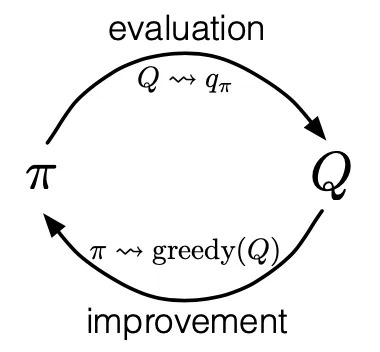
\includegraphics[height=5cm,width=\linewidth,keepaspectratio]{Pictures/deep-reinforcement-learning/gpi-1.jpg}
            \caption{GPI}
        \end{figure}
    \end{minipage}
    \hfill
    \begin{minipage}{0.65\linewidth}
        \begin{figure}[H]
            \centering
            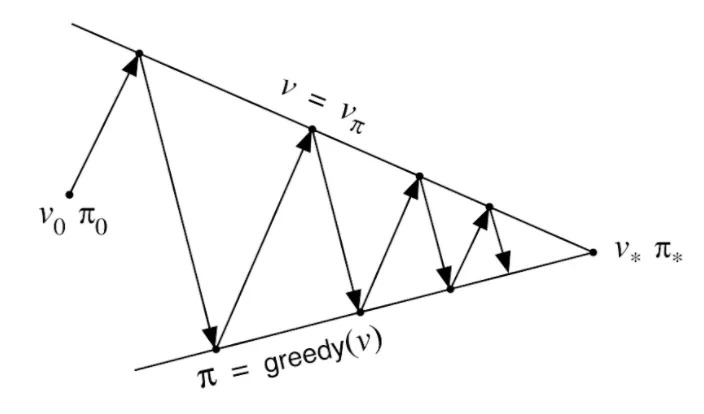
\includegraphics[height=5cm,width=\linewidth,keepaspectratio]{Pictures/deep-reinforcement-learning/gpi-2.jpg}
            \caption{GPI Convergence}
        \end{figure}
    \end{minipage}
\end{table}


\begin{table}[h]
    \centering
    \begin{tabular}{|l|p{5cm}|p{5cm}|}
        \hline
        \textbf{Aspect} & \textbf{Policy Iteration} & \textbf{Generalized Policy Iteration (GPI)} \\
        \hline
        \textbf{Steps} & 
        \tableitemize{
            \item Policy Evaluation
            \item Policy Improvement
        } & 
        \tableitemize{
            \item Policy Evaluation (or Estimation)
            \item Policy Improvement (or Control)
        } \\
        \hline
        \textbf{Step Completion} & 
        Each step is performed to completion before moving to the next. & 
        Steps can be interleaved and performed partially. \\
        \hline
        \textbf{Flexibility} & 
        Less flexible, as it requires full policy evaluation before improvement. & 
        More flexible, allowing for incremental and simultaneous evaluation and improvement. \\
        \hline
        \textbf{Convergence} & 
        Has well-defined convergence criteria. & 
        Requires more sophisticated analysis for convergence, especially with incremental or stochastic steps. \\
        \hline
        \textbf{Practical Use} & 
        Suitable for small state and action spaces where exact solutions are feasible. & 
        Suitable for large-scale or complex problems where exact evaluation and improvement are infeasible. \\
        \hline
        \textbf{Example Algorithms} & 
        Classical Policy Iteration & 
        Q-learning, SARSA \\
        \hline
    \end{tabular}
    \caption{Comparison of Policy Iteration and Generalized Policy Iteration (GPI)}
\end{table}


\section{Monte Carlo (MC)}\label{Monte Carlo (MC)}
Still assuming underlying Markov Decision Process (MDP), but model and reward function are unknown. Agent \textbf{MUST} interact with the environment to learn.

\begin{enumerate}
    \item Monte Carlo methods are a broad class of computational algorithms that rely on repeated random sampling to obtain numerical results.

    \item The underlying concept is to obtain unbiased samples from a complex/ unknown distribution through a random process.

    \item Monte Carlo is a general term that is often used for any estimation method definition which involves a significant random component, however, with respect to Reinforcement Learning, this simply refers to methods that are based on averaging the complete returns. \cite{medium/nerd-for-tech/monte-carlo-methods-for-reinforcement-learning-d30d874dd817}

    \item Monte Carlo methods in reinforcement learning belong to a class of methods that do not assume the knowledge of the model/environment, the agent instead works with the experience the agent gains while it interacts with the environment, which can be an actual environment or a simulated one. \cite{medium/nerd-for-tech/monte-carlo-methods-for-reinforcement-learning-d30d874dd817}
    
    \item Although for training in a simulated environment, we would need some information about the model to simulate the environment, however, it would be much less exhaustive than what we need in techniques like Dynamic Programming, which requires us to know the probabilities of each and every transition. \cite{medium/nerd-for-tech/monte-carlo-methods-for-reinforcement-learning-d30d874dd817}

    \item Monte Carlo methods are based on averaging complete returns, and to ensure that those complete returns are available, Monte Carlo methods are generally defined for episodic tasks, which means that only on the completion of an episode, is the value of the state estimated and policy updated. \cite{medium/nerd-for-tech/monte-carlo-methods-for-reinforcement-learning-d30d874dd817}

\end{enumerate}

\subsection{Monte Carlo Prediction (MC Prediction) \cite{medium/nerd-for-tech/monte-carlo-methods-for-reinforcement-learning-d30d874dd817}} \label{Monte Carlo Prediction}

Prediction refers to the problem of estimating the values of states, a value of a state is an indication of how good is that state for an agent in the given environment, the higher the value of the state the better it is to be in that state.

An obvious way to estimate the value of a state is to simply average all the returns that are observed after a visit to the state, and as we visit the state more often, the average return will converge to the true value of the state in expectation.

\begin{enumerate}
    \item Both first-visit and every-visit Monte Carlo methods converge to true state values when we visit each state many times.

    \item Monte Carlo is one of the few methods in reinforcement learning that do not bootstrap. \textbf{Bootstrapping}\label{RL: Bootstrapping} means making use of estimates to make a further estimations.

    \item In Monte Carlo methods, an estimate of the value of a state does not depend on the estimate of the other state's value rather estimate of each state is independent of each other, although this is beneficial as it reduces the bias, however, it makes convergence significantly slower, as a result of which Monte Carlo methods are seldom used in practical applications.

    \item 

\end{enumerate} 

\vspace{0.2cm}
\textbf{Example}: Consider an MDP with a single nonterminal state and a single action that transitions back to the nonterminal state with probability $p$ and transitions to the terminal state with probability $1-p$. Let the reward be $+1$ on all transitions, and let $\gamma=1$. Suppose you observe one episode that lasts $10$ steps, with a return of $10$. What are the first-visit and every-visit estimators of the value of the nonterminal state?

\subsubsection{First Visit Monte Carlo (first-visit MC) \cite{medium/nerd-for-tech/monte-carlo-methods-for-reinforcement-learning-d30d874dd817}}

In the first visit Monte Carlo methods we average all the rewards observed after the first visit to the state.

\begin{algorithm}[h!]
    \caption{First-Visit Monte Carlo prediction, for estimating $V \approx v_\pi$}

    \textbf{Input}: a policy $\pi$ to be evaluated\\

    \textbf{Initialize}:
    $V(s) \in \mathbb{R} \text{ } \forall s \in S$\\
    $Returns(s) \leftarrow \text{ an empty list,} \forall s\in S$\\

    \ForEach{episode}{
        \While{true}{
            Generate an episode following $\pi: S_0,A_0,R_1,S_1,A_1,R_2,...,S_{T-1},A_{T-1},R_T$\\
            $G \leftarrow 0$\\
            \ForEach{step of episode $t=T-1,T-2,...,0$}{
                $G\leftarrow \gamma G + R_{t+1}$\;
                \Repeat{$S_t$ appears in $S_0,S_1,...,S_{t-1}$}{
                    Append $G$ to $Returns(S_t)$\;
                    $V(S_t) \leftarrow \rcmdXaverage(Returns(S_t))$\;
                }
            }
        }
    }
\end{algorithm}


As per Example, First-visit estimator: $V(s) = 10$


\subsubsection{Every Visit Monte Carlo (every-visit MC) \cite{medium/nerd-for-tech/monte-carlo-methods-for-reinforcement-learning-d30d874dd817}}

In every visit Monte Carlo methods we average the returns following all visits to the state.


As per Example, Every-visit estimator: $V(s) = (10+9+8+7+6+5+4+3+2+1)/10 = 5.5$


\subsection{Monte Carlo Control (MC Control) \cite{medium/nerd-for-tech/monte-carlo-methods-for-reinforcement-learning-d30d874dd817}}

Control problem refers to the problem of estimating optimal policies, because, in situations where the model information is avaliable, state values are sufficient to determine a policy because we know all transition probabilities, however when the model information is not available one must explicitly estimate the value of each action in the state in order for those values to be useful in suggesting a policy.

The only problem being that some of the action-state pairs may not be visited ever, this problem is part of the general problem of \textbf{maintaining sufficient exploration in reinforcement learning}, one of the naive approach that is often taken is called the \textbf{assumption of exploring starts}, which states that every state-action pair has a non-zero probability of being selected as the starting state \& action of the episode, although this does satisfy our requirement of visiting every state \& action pair, it is quite evident that this does not solve the problem of exploration since start states are not very relevant to the outcome of the entire episode.

Optimal policy estimation in Monte Carlo, is based on the general method of \textbf{Generalized Policy Iteration (GPI)} (SEE: \fullref{Generalized Policy Iteration (GPI)}), where the value function is repeatedly altered to more closely approximate the value function for the current policy, and the policy is repeatedly improved with respect to the current value function.

We perform policy evaluation and then subsequently policy improvement repeatedly till we converge and find the optimal policy.

Policy evaluation is done by experiencing many episodes (assuming the episodes are generated with exploring starts) as a result of which the approximate action value function approaches the true function asymptotically, policy improvement is done by making the policy greedy with respect to the current value function.

One critical assumption is that policy evaluation will have to run for an \textbf{infinite} number of episodes for it to actually converge to the true value function.

\subsubsection{on-policy learning \cite{medium/nerd-for-tech/monte-carlo-methods-for-reinforcement-learning-d30d874dd817}}\label{RL: on-policy learning}

These attempt to evaluate or improve the policy that is used to make decisions, however that is actually a compromise - it learns action values not for the optimal policy, but for a near-optimal policy that still explores.


\begin{algorithm}[h!]
    \caption{On-policy first-visit Monte Carlo Control (for $\epsilon$-soft policies), estimates $\pi \approx \pi_*$}

    \textbf{Initialize}: \\
    \ForEach{$s\in S, a\in A(s)$}{
        $Q(s,a) \leftarrow$ arbitrary\\
        $Returns(s,a) \leftarrow$ empty list\\
        $\pi(a|s) \leftarrow$ an arbitrary $\epsilon$-soft policy\\
    }

    \While{true}{
        Generate an episode using $\pi$\\
        \ForEach{pair $s,a$ appearing in the episode}{
            $G\leftarrow$ the return that follows the first occurence of $s,a$\\
            Append $G$ to $Returns(s,a)$\\
            $Q(s,a) \leftarrow average(Returns(s,a))$\\
        }
        
        \ForEach{$s$ in the episode}{
            $A^* \leftarrow \displaystyle\arg\max_a Q(s,a)$ (with ties broken arbitrarily)\\
            \ForEach{$a\in A(s)$}{
                \( \pi(a|s) \leftarrow \begin{cases}
                    1-\epsilon + \displaystyle\dfrac{\epsilon}{|A(s)|} & \text{ if } a=A^*\\
                    \displaystyle\dfrac{\epsilon}{|A(s)|} & \text{ if } a\neq A^*\\
                \end{cases} \)
            }
        }
    }
\end{algorithm}


\subsubsection{off-policy learning \cite{medium/nerd-for-tech/monte-carlo-methods-for-reinforcement-learning-d30d874dd817}}\label{RL: off-policy learning}

A more straightforward approach is to use two policies:
\begin{enumerate}
    \item \textbf{target policy}: one that is learned about and that becomes the optimal policy
    \item \textbf{behavior policy}: one that is more exploratory and is used to generate behavior. 
\end{enumerate}

In this case, we say that learning is from data “off” the target policy, and the overall process is termed \textbf{off-policy learning}.


\begin{enumerate}
    \item we would like to use observations drawn from some policy $b$ to evaluate $q_\pi$ where $\pi \neq b$, specifically, we want to evaluate $q_\pi *$
    \item we strive for full utilization of previous experience
    \item off-policy learning allows us to optimize a \textbf{target policy} while following another \textbf{behavior policy}.
    \item \textbf{Pros}: sample efficient
    \item \textbf{Cons}: greater variance in value estimations
\end{enumerate}

\vspace{0.3cm}
\textbf{Off-policy learning conditions}:
\begin{enumerate}
    \item \textbf{Objective}: use episodes from $b$ to estimate values for $\pi$
    \item For off-policy learning, we must assume coverage:
    \[
        \forall s,a, \text{ } \pi(a|s)>0 \Rightarrow b(a|s) > 0
    \]
    \item if coverage is \textbf{true}, then by running $b$ repeatedly we will eventually discover all possible trajectories for $\pi$
    \item if coverage is \textbf{violated} for some $s,a$, then no inference is possible regarding that state-action value.
\end{enumerate}

\vspace{0.3cm}
\textbf{Trajectory probability}
\begin{enumerate}
    \item An agent following policy $b$ sampled the following trajectory:
    \[
        \tau = {S_0,A_0,R_1,...A_{T-1},R_T,S_T}
    \]
    \[
        Pr(\tau|b) = \displaystyle\sum_{K=0}^{T-1} b(A_K|S_K)p(S_{K+1}|S_K,A_K) 
    \]
    \item but $p(S_{K+1}|S_K,A_K)$ is unknown! so, $Pr(\tau|b)$ cannot be computed!
    \item Assuming MC Control:
    \begin{enumerate}
        \item \(G_t = \displaystyle\sum_{k=t+1}^{T} \gamma^{k-t+1}R_k\)
        \item Append $G_t$ to $Returns(S_t,A_t)$
        \item $Q_b(S_t,A_t) \leftarrow \rcmXWeightedAVG(Returns(S_t,A_t))$ \hfill \( \left( \displaystyle \mathbb{E}[X \sim p] = \sum_x p(x)x \right) \)
        \item Computing the weighted average based on the sample probability would reduce variance (eliminate impact of noisy sampling)
    \end{enumerate}
    
\end{enumerate}


\section{Importance Sampling (IS) \cite{medium/nerd-for-tech/monte-carlo-methods-for-reinforcement-learning-d30d874dd817,bits-pilani-slides}}\label{Importance Sampling (IS)}

Almost all off-policy learning methods utilize \textbf{importance sampling}, a general technique for estimating expected values under one distribution given samples from another. We apply importance sampling to off-policy learning by weighting returns according to the relative probability of their trajectories occurring under the target and behavior policies, called the \textbf{importance-sampling ratio} \indexlabel{importance-sampling ratio}.

\begin{enumerate}
    \item Given a trajectory $\tau$ drawn by running $b$
    \item we can define (not compute) the probability $Pr\{\tau|b\}$
    \item we can also define $Pr\{\tau|\pi\}$
    \item define the importance sampling ratio as $\rho_t = \displaystyle\dfrac{Pr\{\tau|\pi\}}{Pr\{\tau|b\}}$
    \item Computing $\rho$ without $p(S_{K+1}|S_K,A_K)$ 
    \[
        \rho_t = \displaystyle\dfrac{Pr\{\tau|\pi\}}{Pr\{\tau|b\}} = \displaystyle\dfrac{\displaystyle\prod_{k=t}^{T-1} \pi(A_k|S_k)\cancel{p(S_{K+1}|S_K,A_K)}}{\displaystyle\prod_{k=t}^{T-1} b(A_k|S_k)\cancel{p(S_{K+1}|S_K,A_K)}} = \displaystyle\prod_{k=t}^{T-1}\displaystyle\dfrac{\pi(A_k|S_k)}{b(A_k|S_k)}
    \]
    \item \textbf{Fact}: \( \mathbb{E}_{\tau \sim b}[G_t|S_t=s]=v_b(s) \)
    \item Importance sampling allows us to compute an unbiased estimate of $v_\pi(s)$ by running $b$.
    \item \textbf{Claim}: \( \mathbb{E}_{\tau \sim b}[\rho_t G_t|S_t=s]=v_\pi(s) \)
    \item We set $v_\pi(s)$ to be a weighted average of observed returns (weighted by the importance ratio).
    \item Assume visiting state $s$ over $M$ episodes using policy $b$
    \item $s$ is first visited during time step $t^m$ during each episode, $m\in M$
    \[
        v_\pi(s) = \displaystyle\dfrac{\displaystyle\sum_{m\in M} \rho_t m G_t^m}{M}
    \]
\end{enumerate}


\subsection{Ordinary Importance Sampling \cite{medium/nerd-for-tech/monte-carlo-methods-for-reinforcement-learning-d30d874dd817}}\label{RL: Ordinary Importance Sampling}

Importance sampling with a simple average is called ordinary sampling.

\[
    V(s) = \displaystyle\dfrac{\displaystyle\sum_{t\in J(s)} \rho_{t:t(t)-1}G_t}{|J(s)|}
\]

\begin{enumerate}
    \item it is unbiased
    \item results in high variance
\end{enumerate}

\subsection{Weighted importance sampling \cite{medium/nerd-for-tech/monte-carlo-methods-for-reinforcement-learning-d30d874dd817}}\label{RL: Weighted importance sampling}

Importance Sampling with a weighted average is known as weighted importance sampling.

\[
    V(s) = \displaystyle\dfrac{\displaystyle\sum_{t\in J(s)} \rho_{t:t(t)-1}G_t}{\displaystyle\sum_{t\in J(s)} \rho_{t:t(t)-1}} \hfill \text{\cite{medium/nerd-for-tech/monte-carlo-methods-for-reinforcement-learning-d30d874dd817}}
\]
\[
    v_\pi(s) = \displaystyle\dfrac{\displaystyle\sum_{m\in M} \rho_t m G_t^m}{\displaystyle\sum_{m\in M} \rho_t m} \hfill \text{\cite{bits-pilani-slides}}
\]

\begin{enumerate}
    \item it is biased (initially)
    \item results in bounded variance
\end{enumerate}

the decision of which one to use when, circles back to the classic bias-variance tradeoff, however in practice, the 
weighted estimator is strongly preferred.

\section{Incremental Monte Carlo (Incremental MC) \cite{redirect.cs.umbc.edu/courses/graduate/678/fall21/RL05}} \label{RL: Incremental Monte Carlo (Incremental MC)}

\begin{enumerate}
    \item Update value without tracking all returns
    
    \item \textbf{Ordinary importance sampling}:
    \[
        V_{n+1} = V_n + \displaystyle\dfrac{1}{n}[W_nG_n - V_n]
    \]

    \item \textbf{Weighted importance sampling:}
    \[
        V_{n+1} = V_n + \displaystyle\dfrac{W_n}{C_n}[G_n - V_n] \hfill \text{(for $n\geq 1$)}
    \]
    \[
        C_{n+1} = C_n + W_{n+1}
    \]
\end{enumerate}

\begin{algorithm}[h!]
    \caption{Off-Policy Monte Carlo Prediction (Policy Evaluation) for estimating $Q \approx q_*$}

    \textbf{Input}: an arbitrary target policy $\pi$\\

    \textbf{Initialize:}\\
    \ForEach{$s\in S, a\in A(s)$}{
        $Q(s,a) \in \mathbb{R}$ (arbitrarily)\\
        $C(s,a) \leftarrow 0$
    }

    \ForEach{episode}{
        \While{true}{
            $b \leftarrow \text{ any policy with coverage of } \pi$\\
            Generate an episode following $b: S_0,A_0,R_1,...,S_{T-1},A_{T-1},R_T$\\
            $G\leftarrow 0$\\
            $W\leftarrow 1$\\
            \ForEach{step of episode $t=T-1,T-2,...,0$}{
                $G \leftarrow \gamma G + R_{t+1}$\\
                $C(S_t,A_t) \leftarrow C(S_t,A_t) + W$\\
                $Q(S_t,A_t) \leftarrow Q(S_t,A_t) + \displaystyle\dfrac{W}{C(S_t,A_t)}|G-Q(S_t,A_t)|$\\
                $W \leftarrow W\displaystyle\dfrac{\pi(A_t|S_t)}{b(A_t|S_t)}$\\
                \If{$W=0$}{
                    exit For loop
                }
            }
        }
    }
\end{algorithm}


\begin{algorithm}[h!]
    \caption{Off-Policy Monte Carlo Control (Policy Improvement) for estimating $\pi \approx \pi_*$}

    \textbf{Initialize:}\\
    \ForEach{$s\in S, a\in A(s)$}{
        $Q(s,a) \in \mathbb{R}$ (arbitrarily)\\
        $C(s,a) \leftarrow 0$\\
        $\pi(s) \leftarrow \displaystyle\arg\max_a Q(s,a)$ (with ties broken consistently)\\
    }

    \ForEach{episode}{
        \While{true}{
            $b \leftarrow$ any soft policy\\
            Generate an episode following $b: S_0,A_0,R_1,...,S_{T-1},A_{T-1},R_T$\\

            \Comment{Accumulated reward at step $t$}
            $G\leftarrow 0$

            \Comment{1 over joint probability over observed actions from following $b$ after step $t$. This equals the IS ratio here because the target policy is deterministic.}
            $W\leftarrow 1$

            \Comment{Going back in time}
            \ForEach{step of episode $t=T-1,T-2,...,0$}{
                \Comment{Discount future rewards and add immediate reward}
                $G \leftarrow \gamma G + R_{t+1}$

                \Comment{Cumulative sum of IS weights affiliated with $S_t,A_t$ (for weighted IS)}
                $C(S_t,A_t) \leftarrow C(S_t,A_t) + W$

                \Comment{Incremental update of Q values (waited moving average)}
                $Q(S_t,A_t) \leftarrow Q(S_t,A_t) + \displaystyle\dfrac{W}{C(S_t,A_t)}|G-Q(S_t,A_t)|$

                \Comment{update target policy (greedy)}
                $\pi(S_t) \leftarrow \displaystyle\arg\max_a Q(S_t,a)$ (with ties broken consistently)

                \Comment{Since $\pi$ is deterministic, once we diverge from it all IS weights of earlier actions will be $0$}
                \If{$A_t \neq \pi(S_t)$}{
                    exit For loop
                }

                \Comment{Update the joint prob by multiplying by $\rho_t$. Notice that $\pi(S_t)=1$ in this example (deterministic target policy).}
                $W \leftarrow W\displaystyle\dfrac{1}{b(A_t|S_t)}$
            }
        }
    }
\end{algorithm}













































































































